\documentclass[11pt,a4paper]{article}

\usepackage[margin=2.6cm]{geometry}
\usepackage[T1]{fontenc}
\usepackage[utf8]{inputenc}
\usepackage{mathptmx}
\usepackage[scaled=0.92]{helvet}
\usepackage{microtype}
\usepackage{amsmath,amssymb,amsthm}
\usepackage{graphicx}
\graphicspath{{../graphs/}}
\usepackage{booktabs}
\usepackage{array}
\usepackage[font=small,labelfont=bf,skip=6pt]{caption}
\usepackage{xcolor}
\usepackage{enumitem}
\usepackage[hidelinks,breaklinks]{hyperref}
\usepackage{url}
\urlstyle{same}

\renewcommand{\topfraction}{0.9}
\renewcommand{\bottomfraction}{0.9}
\renewcommand{\textfraction}{0.05}
\renewcommand{\floatpagefraction}{0.85}
\setcounter{topnumber}{3}
\setcounter{totalnumber}{4}
\setlength{\parskip}{5pt}
\setlength{\parindent}{0pt}
\linespread{1.06}

\theoremstyle{plain}
\newtheorem{theorem}{Theorem}[section]
\newtheorem{lemma}[theorem]{Lemma}
\newtheorem{corollary}[theorem]{Corollary}
\theoremstyle{definition}
\newtheorem{definition}[theorem]{Definition}
\newtheorem{example}[theorem]{Example}

\newcommand{\regret}{\mathrm{Regret}}
\newcommand{\E}{\mathbb{E}}
\newcommand{\N}{\mathbb{N}}
\newcommand{\R}{\mathbb{R}}
\newcommand{\sq}[1]{\sqrt{#1}}
\newcommand{\repo}{https://github.com/bental1/MW-Seminar}
\newcommand{\script}[1]{\small\texttt{graphs/#1} --- \url{\repo/blob/main/graphs/#1}}

\begin{document}

% ------------------------------------------------------------------ title page
\begin{titlepage}
\pagenumbering{gobble}
\vspace*{2.2cm}
{\Huge\bfseries Seminar 20954\par}
\vspace{0.6cm}
{\Large\bfseries The Multiplicative Weights Update Method:\\A Meta-Algorithm and Applications\par}
\vspace{0.4cm}
{\large Arora, Hazan and Kale, \emph{Theory of Computing} 8 (2012), 121--164 \cite{AHK12}\par}
\vspace{0.2cm}
\url{https://theoryofcomputing.org/articles/v008a006/v008a006.pdf}

\vfill
{\large
\textbf{By:} Tal Idelson\\[3pt]
\textbf{Supervised by:} Prof.\ Zeev Nutov\\[3pt]
Computer Science, The Open University of Israel\\[12pt]
\textbf{Code and figures:} \url{\repo} \cite{Repo}\\
Every figure in this document was generated by a script in that repository; the caption of each figure names the script and gives its direct URL.
}
\end{titlepage}
\pagenumbering{arabic}

\tableofcontents
\clearpage

% ================================================================== 1
\section{Introduction}

\subsection{The problem}
\label{sec:problem}

The survey studies one abstract game, played for $T$ rounds between an algorithm and an adversary.

\begin{definition}[Online decision problem with $n$ decisions]
\label{def:problem}
Fix $n \ge 2$ decisions and a horizon $T \ge 1$. In every round $t = 1,\dots,T$:
\begin{enumerate}[nosep]
  \item the algorithm chooses a probability distribution $p^{(t)} = (p^{(t)}_1,\dots,p^{(t)}_n)$, $p^{(t)}_i \ge 0$, $\sum_i p^{(t)}_i = 1$;
  \item the adversary, after seeing $p^{(t)}$, reveals a cost vector $m^{(t)} \in [-1,1]^n$;
  \item the algorithm pays the expected cost $m^{(t)}\cdot p^{(t)} = \sum_{i=1}^n p^{(t)}_i m^{(t)}_i$.
\end{enumerate}
The \emph{regret} of the algorithm after $T$ rounds is
\begin{equation}
\label{eq:regret}
\regret_T \;=\; \sum_{t=1}^{T} m^{(t)}\cdot p^{(t)} \;-\; \min_{i}\, \sum_{t=1}^{T} m^{(t)}_i ,
\end{equation}
the cost it actually paid, minus the cost of the best \emph{single} decision, chosen with hindsight and held fixed for all $T$ rounds. The goal is an algorithm whose regret is $o(T)$ for \emph{every} cost sequence, i.e.\ $\regret_T / T \to 0$ as $T \to \infty$.
\end{definition}

The two results of the survey that this seminar proves answer this problem from both sides. For the Multiplicative Weights algorithm of Section~\ref{sec:algorithm}, on \emph{every} cost sequence, whenever $T \ge 4\ln n$ (Theorem~\ref{thm:mw} with the best $\eta$),
\begin{equation}
\label{eq:upper}
\regret_T \;\le\; 2\sq{T\ln n}\,;
\end{equation}
and for \emph{every} algorithm there is \emph{some} cost sequence (Theorem~\ref{thm:lower}) on which its expected regret satisfies
\begin{equation}
\label{eq:lower}
\regret_T \;\ge\; \tfrac{1}{80}\sq{T\ln(n-1)}\,.
\end{equation}
Together: the optimal regret is $\Theta(\sq{T\ln n})$, and the four-line algorithm of Section~\ref{sec:algorithm} achieves it.

\begin{figure}[htbp]
\centering
\includegraphics[width=\textwidth]{setting_all.png}
\caption{The problem of Definition~\ref{def:problem} in one picture: $n$ decisions on the left; one round in the middle (we choose $p^{(t)}$, the adversary sees it and sets $m^{(t)}$, we pay $m^{(t)}\cdot p^{(t)}$), repeated $T$ times; the yardstick on the right.\\ \script{setting\_plot.py}}
\label{fig:setting}
\end{figure}

\paragraph{What the definition says in words.}
The $n$ decisions can be anything: stocks to hold, experts to follow, routes to take, constraints to satisfy. Each round we do not pick one of them; we spread our bets, and $p^{(t)}$ says how. Only after we have committed does the round's cost of every decision appear, and we pay the average cost under our bets. A negative cost is a gain.

Three features make the problem hard, and each is deliberate.
First, nothing is promised about the costs: no distribution, no pattern, no fairness. They may be chosen by an adversary who knows our algorithm and sees $p^{(t)}$ before choosing $m^{(t)}$. This is why we bet a distribution rather than a single decision --- a single fixed choice could be made expensive every round, while a spread of bets gives the adversary nothing fixed to aim at.
Second, the yardstick is not the best \emph{sequence} of choices --- against an adversary that is hopeless --- but the best single decision in hindsight. The difference, the regret, is the price we pay for not knowing the future.
Third, the regret is allowed to grow with $T$; it is the cost of learning. What is demanded is that it grow \emph{slower} than $T$, so that per round we end up as good as the best single decision without ever knowing which one it was.

\subsection{Predecessors: one update rule, found three times}

The algorithmic idea behind the survey --- keep a weight on every decision and multiply it by a factor set by its cost --- was discovered independently in at least three fields before the survey unified them \cite[Section~1]{AHK12}:
\begin{itemize}[nosep]
  \item \emph{Learning theory} (1988): Littlestone's Winnow algorithm \cite{Littlestone88} multiplies the weight of a feature by a constant whenever a mistake is made, and learns linear threshold functions with a mistake bound that is logarithmic in the number of irrelevant features.
  \item \emph{Optimization} (1991): Plotkin, Shmoys and Tardos \cite{PST95} decide the feasibility of fractional packing and covering linear programs approximately, by keeping a weight on every constraint and increasing the weight of the constraints the current point violates.
  \item \emph{Boosting} (1997): Freund and Schapire's AdaBoost \cite{FS97} keeps a weight on every training example and shrinks the weights of the examples the current hypothesis classifies correctly, so that the next weak learner concentrates on the hard ones.
\end{itemize}
Each line of work had its own notation, its own proof and its own community; the observation that they are literally the same update rule was, in the authors' words, ``clear to several researchers'' but never written down as one theorem \cite[p.~122]{AHK12}. Section~\ref{sec:examples} shows two of these instantiations side by side, and Section~\ref{sec:nature} a third one that comes from outside computer science.

\subsection{What the survey contributes}

The contribution is of two kinds.
\emph{Organisational}: a single Multiplicative Weights (MW) meta-algorithm with a single potential-function proof (Theorem~\ref{thm:mw}), from which Weighted Majority, Hedge, Winnow, the Plotkin--Shmoys--Tardos framework, AdaBoost and the approximate solution of zero-sum games all follow by choosing what a decision is, what its cost is, and the rate $\eta$ (Figure~\ref{fig:template}).
\emph{Technical}: a few results that were new at the time, among them a variant of the Garg--K\"onemann multicommodity-flow algorithm \cite[Section~3.4]{AHK12}, and the matching lower bound (Theorem~\ref{thm:lower}) showing that the $\sq{T\ln n}$ term in the regret bound cannot be improved by \emph{any} online algorithm \cite[Section~4]{AHK12}.

\begin{figure}[htbp]
\centering
\includegraphics[width=0.92\textwidth]{template_plot.png}
\caption{A meta-algorithm is a template with four empty slots. Filling the slots produces AdaBoost, the Plotkin--Shmoys--Tardos algorithm, and (Section~\ref{sec:nature}) the dynamics of natural selection.\\ \script{template\_plot.py}}
\label{fig:template}
\end{figure}

% ================================================================== 2
\clearpage
\section{Structure of the survey}

The survey \cite{AHK12} builds from one concrete example to the general algorithm, its applications and its limits.
\emph{Section~1} motivates the method with the Weighted Majority algorithm for binary prediction: each expert starts with equal weight, an expert that errs has its weight multiplied by $(1-\eta)$, and the algorithm follows the weighted majority; a first bound (Theorem~1.1) is proved before any general machinery.
\emph{Section~2} is the heart: $n$ decisions, costs in $[-1,1]$ chosen adversarially, the MW update $w^{(t+1)}_i = w^{(t)}_i(1-\eta m^{(t)}_i)$ and its exponential cousin Hedge, $w^{(t+1)}_i = w^{(t)}_i e^{-\eta m^{(t)}_i}$, both with a guarantee of the form of Theorem~\ref{thm:mw}.
\emph{Section~3} is a sequence of applications, each obtained by choosing decisions and costs inside the framework: zero-sum games, linear programs, flows, boosting, hard-core sets, and more.
\emph{Section~4} asks whether the analysis can be improved and answers no, by the probabilistic method (our Section~\ref{sec:lower}).
\emph{Section~5} generalises weights to density matrices, giving the Matrix Multiplicative Weights algorithm behind semidefinite-programming applications.

This seminar covers Sections 1, 2 and 4 in full (Sections~\ref{sec:algorithm}--\ref{sec:lower}), two applications from Section~3 (Section~\ref{sec:examples}), an application from biology that cites the survey (Section~\ref{sec:nature}), and a look at what has been built on the survey since (Section~\ref{sec:influence}).

% ================================================================== 3
\clearpage
\section{The algorithm}
\label{sec:algorithm}

The Multiplicative Weights algorithm is four lines \cite[Section~2.1]{AHK12}. It has one free parameter, the learning rate $\eta \le \tfrac12$.

\begin{center}
\begin{tabular}{@{}ll@{}}
\toprule
initialise & $w^{(1)}_i = 1$ for every decision $i = 1,\dots,n$\\[2pt]
\midrule
\multicolumn{2}{@{}l}{each round $t = 1,\dots,T$:}\\[2pt]
\quad play & decision $i$ with probability $p^{(t)}_i = w^{(t)}_i / \Phi^{(t)}$, where $\Phi^{(t)} = \sum_{j} w^{(t)}_j$\\[2pt]
\quad observe & the cost vector $m^{(t)} \in [-1,1]^n$\\[2pt]
\quad update & $w^{(t+1)}_i = w^{(t)}_i\,\bigl(1 - \eta\, m^{(t)}_i\bigr)$ for every $i$\\
\bottomrule
\end{tabular}
\end{center}

Each line has a job, and only one of them learns. The initialisation means ``no opinion'': every decision equally credible. The play line backs each decision in proportion to how it has done. The observe line is where the adversary moves. The update line shrinks a weight in proportion to its own cost: a decision that cost $1$ loses a fraction $\eta$ of its weight, a decision that cost $0$ keeps it, a decision with negative cost gains. Because the factor $1-\eta m_i$ is never zero (since $\eta \le \frac12$ and $|m_i| \le 1$), losers decay exponentially but no decision is ever written off completely --- which is exactly what an adversary who might revive a decision later requires.

Figure~\ref{fig:stocks} shows a run on four stocks. Two of them crash in turn; the probability mass drains out of the losers within a few rounds and pools on the one that keeps gaining, without anyone having told the algorithm which stock that would be.

\begin{figure}[htbp]
\centering
\includegraphics[width=\textwidth]{stock_plot.png}
\caption{A worked run of MW: $n=4$ stocks, $T=16$ days, $\eta=0.4$. Left: cumulative cost of each stock (AutoCo crashes on day 5, RetailCo on day 9). Right: the distribution $p^{(t)}$ over the days.\\ \script{stock\_plot.py}}
\label{fig:stocks}
\end{figure}

% ================================================================== 4
\clearpage
\section{The proof of the regret bound}
\label{sec:proof}

\begin{theorem}[{\cite[Theorem~2.1]{AHK12}}]
\label{thm:mw}
Let $\eta \le \frac12$ and let all costs lie in $[-1,1]$. After $T$ rounds of the Multiplicative Weights algorithm, for \emph{every} decision $i$,
\begin{equation}
\label{eq:thm}
\sum_{t=1}^{T} m^{(t)}\cdot p^{(t)} \;\le\; \sum_{t=1}^{T} m^{(t)}_i \;+\; \eta \sum_{t=1}^{T} \bigl|m^{(t)}_i\bigr| \;+\; \frac{\ln n}{\eta}.
\end{equation}
\end{theorem}

The left side is what the algorithm paid. The right side is what decision $i$ paid, plus two correction terms. Since the statement holds for every $i$ at once, it holds in particular for the best decision in hindsight, which is how it becomes a regret bound (Section~\ref{sec:bound}).

\subsection{The method: one quantity both sides control}

The two quantities we want to compare live in different worlds: the algorithm's cost depends on distributions that change every round, while the benchmark is a single decision that never moves. They cannot be compared directly. The proof finds one quantity that both of them control --- the total weight, the \emph{potential}
\[
\Phi^{(t)} \;=\; \sum_{j=1}^{n} w^{(t)}_j ,
\]
and bounds it from below (using decision $i$'s costs) and from above (using the algorithm's costs). Squeezing the two bounds together and taking logarithms gives the theorem.

\subsection{The easy half: a lower bound on \texorpdfstring{$\Phi$}{Phi}}

All weights stay positive (each factor $1-\eta m^{(t)}_i \ge \frac12$), so the total is at least any single term:
\[
w^{(T+1)}_i \;\le\; \Phi^{(T+1)} \qquad\text{for every decision } i .
\]
Unrolling decision $i$'s own updates from $w^{(1)}_i = 1$,
\begin{equation}
\label{eq:lowerPhi}
\prod_{t=1}^{T}\bigl(1-\eta\, m^{(t)}_i\bigr) \;=\; w^{(T+1)}_i \;\le\; \Phi^{(T+1)} .
\end{equation}
This side depends only on decision $i$'s costs and says nothing about what the algorithm did.

\subsection{The harder half: an upper bound on \texorpdfstring{$\Phi$}{Phi}}

Substitute the update rule into the definition of $\Phi$, then $w^{(t)}_i = p^{(t)}_i \Phi^{(t)}$:
\[
\Phi^{(t+1)} \;=\; \sum_i w^{(t)}_i\bigl(1-\eta m^{(t)}_i\bigr)
\;=\; \Phi^{(t)} - \eta\sum_i w^{(t)}_i m^{(t)}_i
\;=\; \Phi^{(t)}\Bigl(1 - \eta\, m^{(t)}\cdot p^{(t)}\Bigr).
\]
This is the crucial step: each round, $\Phi$ is multiplied by a factor governed exactly by the algorithm's expected cost that round. It shrinks when we pay and grows when we gain. Using $1-x \le e^{-x}$ (valid for every real $x$),
\[
\Phi^{(t+1)} \;\le\; \Phi^{(t)}\, e^{-\eta\, m^{(t)}\cdot p^{(t)}},
\]
and chaining this over all $T$ rounds, starting from $\Phi^{(1)} = n$,
\begin{equation}
\label{eq:upperPhi}
\Phi^{(T+1)} \;\le\; n\, \exp\Bigl(-\eta \sum_{t=1}^{T} m^{(t)}\cdot p^{(t)}\Bigr).
\end{equation}
The exponential form is chosen because it telescopes: a product of $T$ factors becomes a single exponential of a sum.

\subsection{The sandwich, and taking logarithms}

Combining \eqref{eq:lowerPhi} and \eqref{eq:upperPhi}, for every decision $i$,
\begin{equation}
\label{eq:sandwich}
\prod_{t=1}^{T}\bigl(1-\eta\, m^{(t)}_i\bigr) \;\le\; \Phi^{(T+1)} \;\le\; n\, \exp\Bigl(-\eta \sum_{t=1}^{T} m^{(t)}\cdot p^{(t)}\Bigr).
\end{equation}
Decision $i$'s costs sit below $\Phi$, the algorithm's costs above it, and $\Phi$ itself can now be forgotten. Figure~\ref{fig:sandwich} shows the three quantities on a real run.

\begin{figure}[htbp]
\centering
\includegraphics[width=0.74\textwidth]{sandwich_plot.png}
\caption{The sandwich \eqref{eq:sandwich} on a simulated run ($n=8$, $T=250$, $\eta=0.1$, costs uniform in $[-1,1]$): the potential $\Phi^{(t)}$ (solid) stays between the best decision's own weight (dashed) and the upper bound $n\,e^{-\eta\sum m\cdot p}$ (dotted). Because costs can be negative, $\Phi$ may rise; both bounds hold regardless.\\ \script{sandwich\_plot.py}}
\label{fig:sandwich}
\end{figure}

Taking logarithms turns the product into a sum and cancels the exponential:
\[
\sum_{t=1}^{T} \ln\bigl(1-\eta\, m^{(t)}_i\bigr) \;\le\; \ln n \;-\; \eta \sum_{t=1}^{T} m^{(t)}\cdot p^{(t)} .
\]
Now use the elementary inequality $\ln(1-z) \ge -z - z^2$, valid for $|z| \le \frac12$, with $z = \eta m^{(t)}_i$ (this is where $\eta \le \frac12$ and $|m^{(t)}_i| \le 1$ are needed):
\[
-\eta\sum_t m^{(t)}_i \;-\; \eta^2 \sum_t \bigl(m^{(t)}_i\bigr)^2 \;\le\; \ln n \;-\; \eta \sum_t m^{(t)}\cdot p^{(t)} .
\]
Rearranging, dividing by $\eta$, and using $(m^{(t)}_i)^2 \le |m^{(t)}_i|$ (since $|m^{(t)}_i| \le 1$) gives \eqref{eq:thm}. \qed

\paragraph{Why the structure generalises.}
Nothing in the proof used how the costs were generated; they may depend on the algorithm's current weights, because $\Phi^{(t)}$ depends only on the past. The same skeleton --- define a potential, bound it above by the update rule, below by non-negativity, compare through logarithms --- reappears with only the potential changed: $e^{-\eta m}$ in place of $1-\eta m$ gives the Hedge bound \cite[Section~2.2]{AHK12}, and replacing $\Phi$ by the relative entropy gives the bound for restricted distributions \cite[Section~2.3]{AHK12}.

% ================================================================== 5
\clearpage
\section{The bound and its limits}
\label{sec:bound}

\subsection{From the theorem to a regret bound}

Theorem~\ref{thm:mw} holds for every $i$, so take $i$ to be the best decision in hindsight. Since costs lie in $[-1,1]$, $|m^{(t)}_i| \le 1$ and $\sum_t |m^{(t)}_i| \le T$. Substituting and moving $\min_i \sum_t m^{(t)}_i$ to the left,
\begin{equation}
\label{eq:regretbound}
\regret_T \;=\; \sum_{t=1}^{T} m^{(t)}\cdot p^{(t)} - \min_i \sum_{t=1}^{T} m^{(t)}_i \;\le\; \eta T + \frac{\ln n}{\eta}.
\end{equation}

\subsection{Choosing \texorpdfstring{$\eta$}{eta}}

The right side of \eqref{eq:regretbound} has two terms pulling in opposite directions: $\eta T$ grows with $\eta$ (a large rate overreacts to every round), $\ln n / \eta$ shrinks with $\eta$ (a small rate learns too slowly). Minimising over $\eta$: $\frac{d}{d\eta}\bigl(\eta T + \ln n/\eta\bigr) = T - \ln n/\eta^2 = 0$ gives
\[
\eta^{*} \;=\; \sq{\frac{\ln n}{T}} , \qquad\text{at which both terms equal } \sq{T\ln n}, \qquad\text{so}\qquad \regret_T \;\le\; 2\sq{T\ln n}.
\]
(The constraint $\eta \le \frac12$ holds as soon as $T \ge 4\ln n$.) This is the upper bound \eqref{eq:upper}. Figure~\ref{fig:eta} shows the two terms and their sum for one choice of $n$ and $T$.

\begin{figure}[htbp]
\centering
\begin{minipage}[t]{0.49\textwidth}
\centering
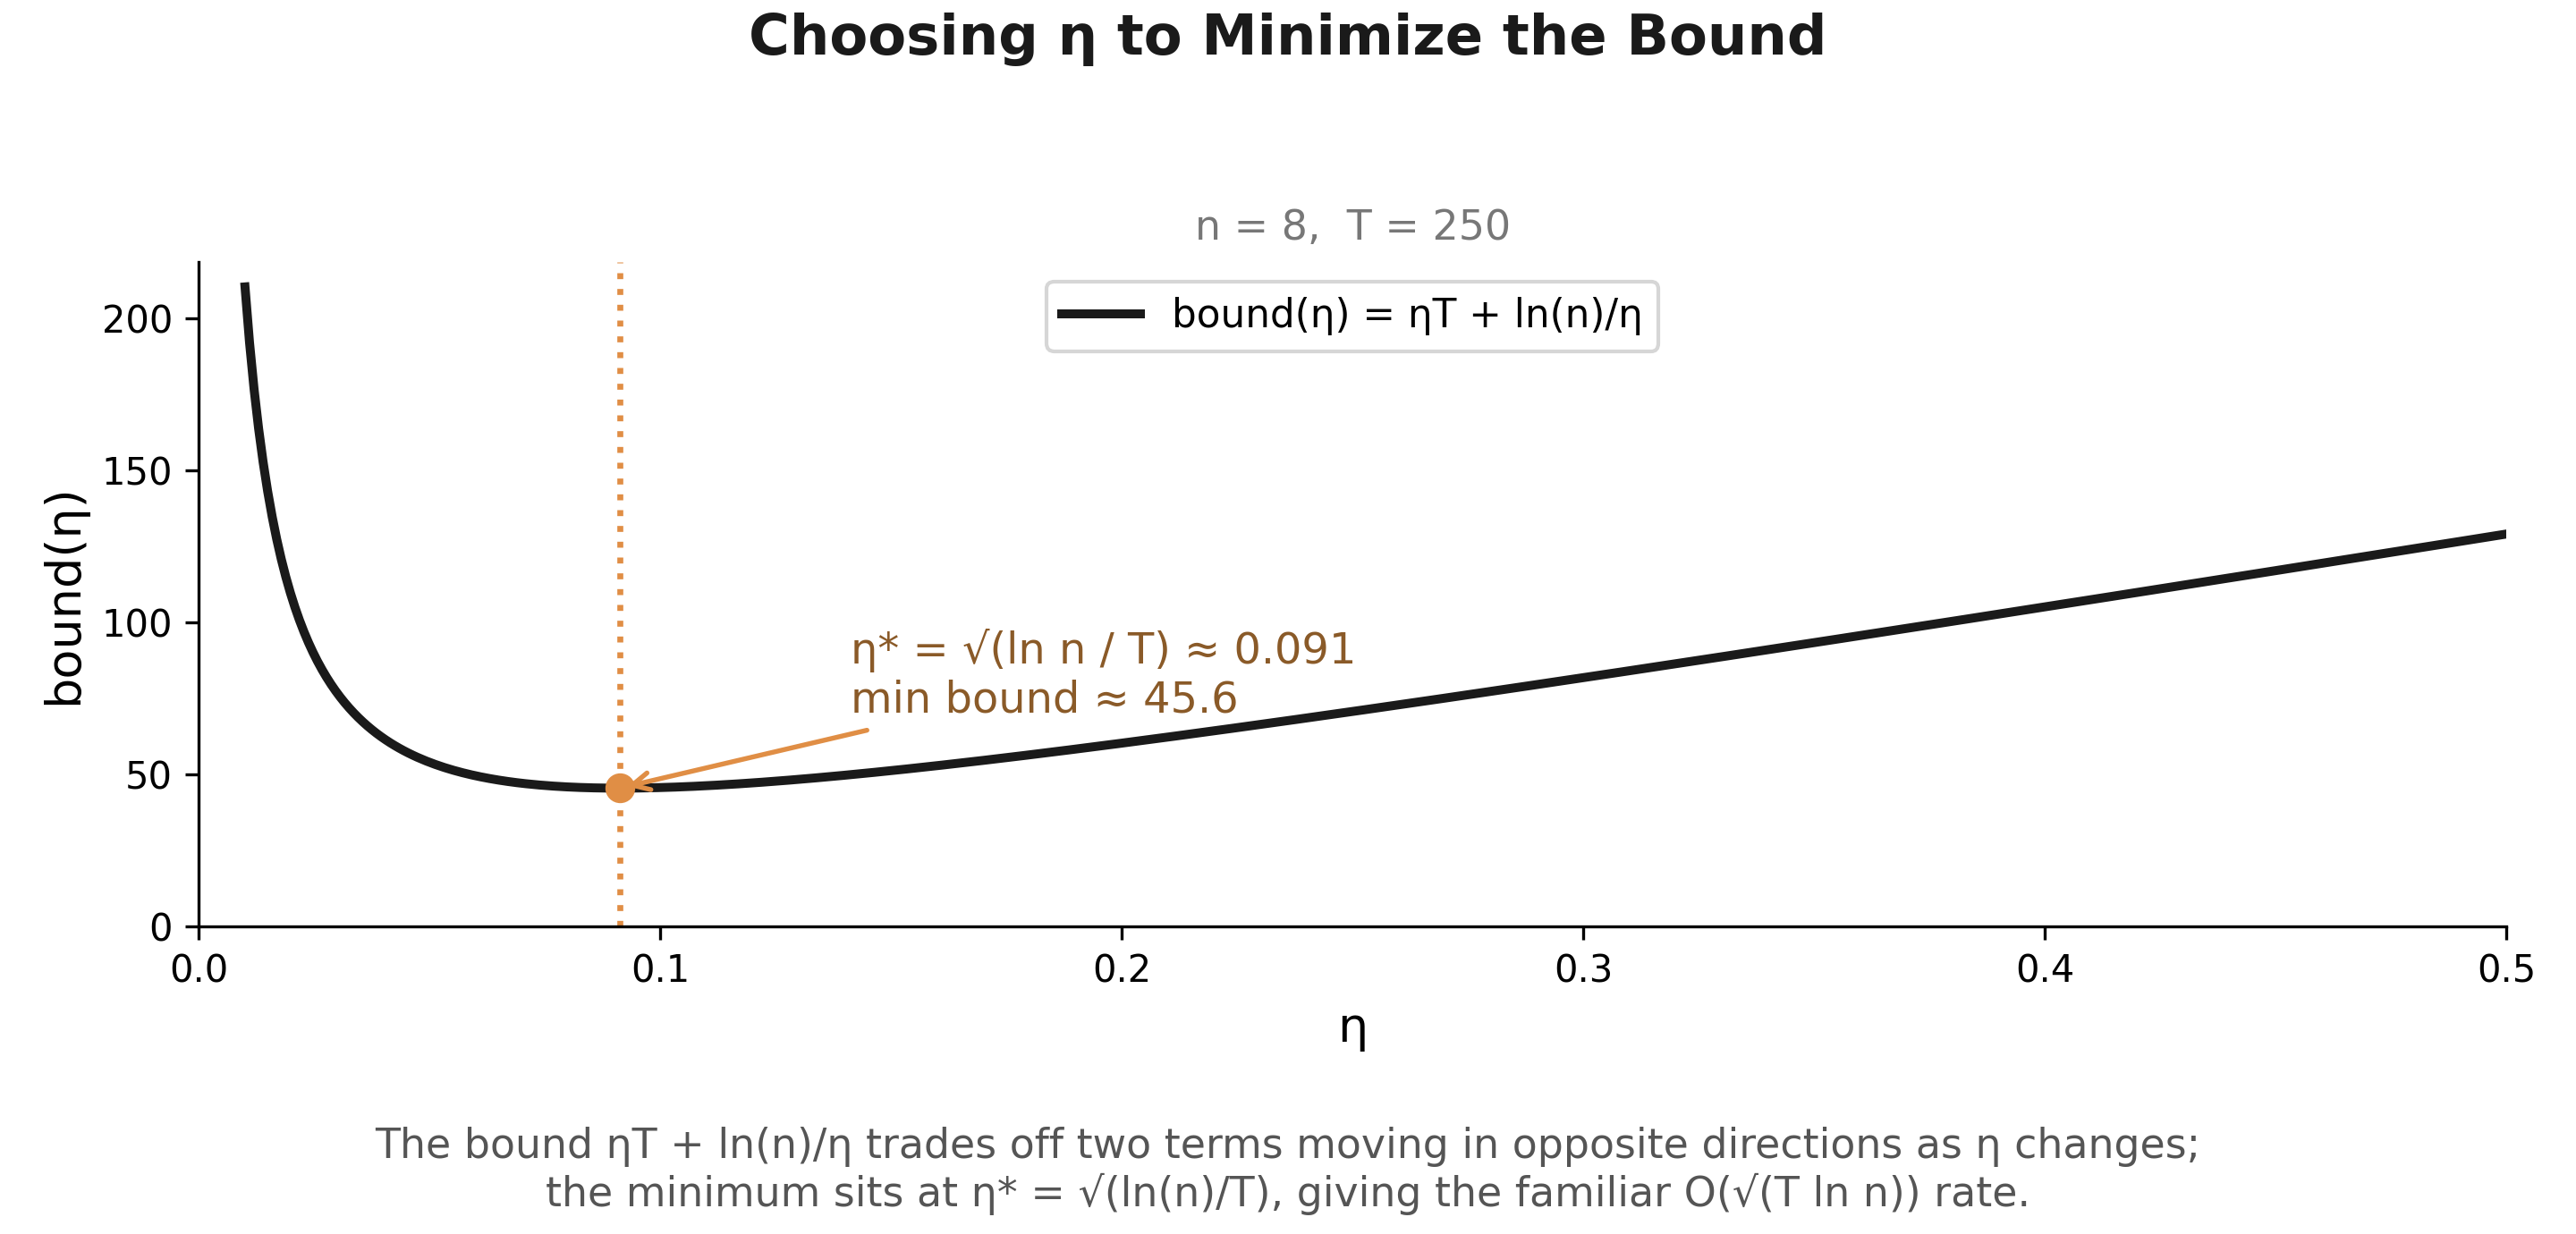
\includegraphics[width=\textwidth]{optimal_eta_plot.png}
\caption{The bound $\eta T + \ln n/\eta$ against $\eta$ for $n=8$, $T=256$: the overreacting term $\eta T$, the slow-learning term $\ln n/\eta$, and their sum, minimised at $\eta^* = \sq{\ln n/T} \approx 0.09$ where the bound equals $2\sq{T\ln n} \approx 46$.\\ \script{optimal\_eta\_plot.py}}
\label{fig:eta}
\end{minipage}\hfill
\begin{minipage}[t]{0.49\textwidth}
\centering
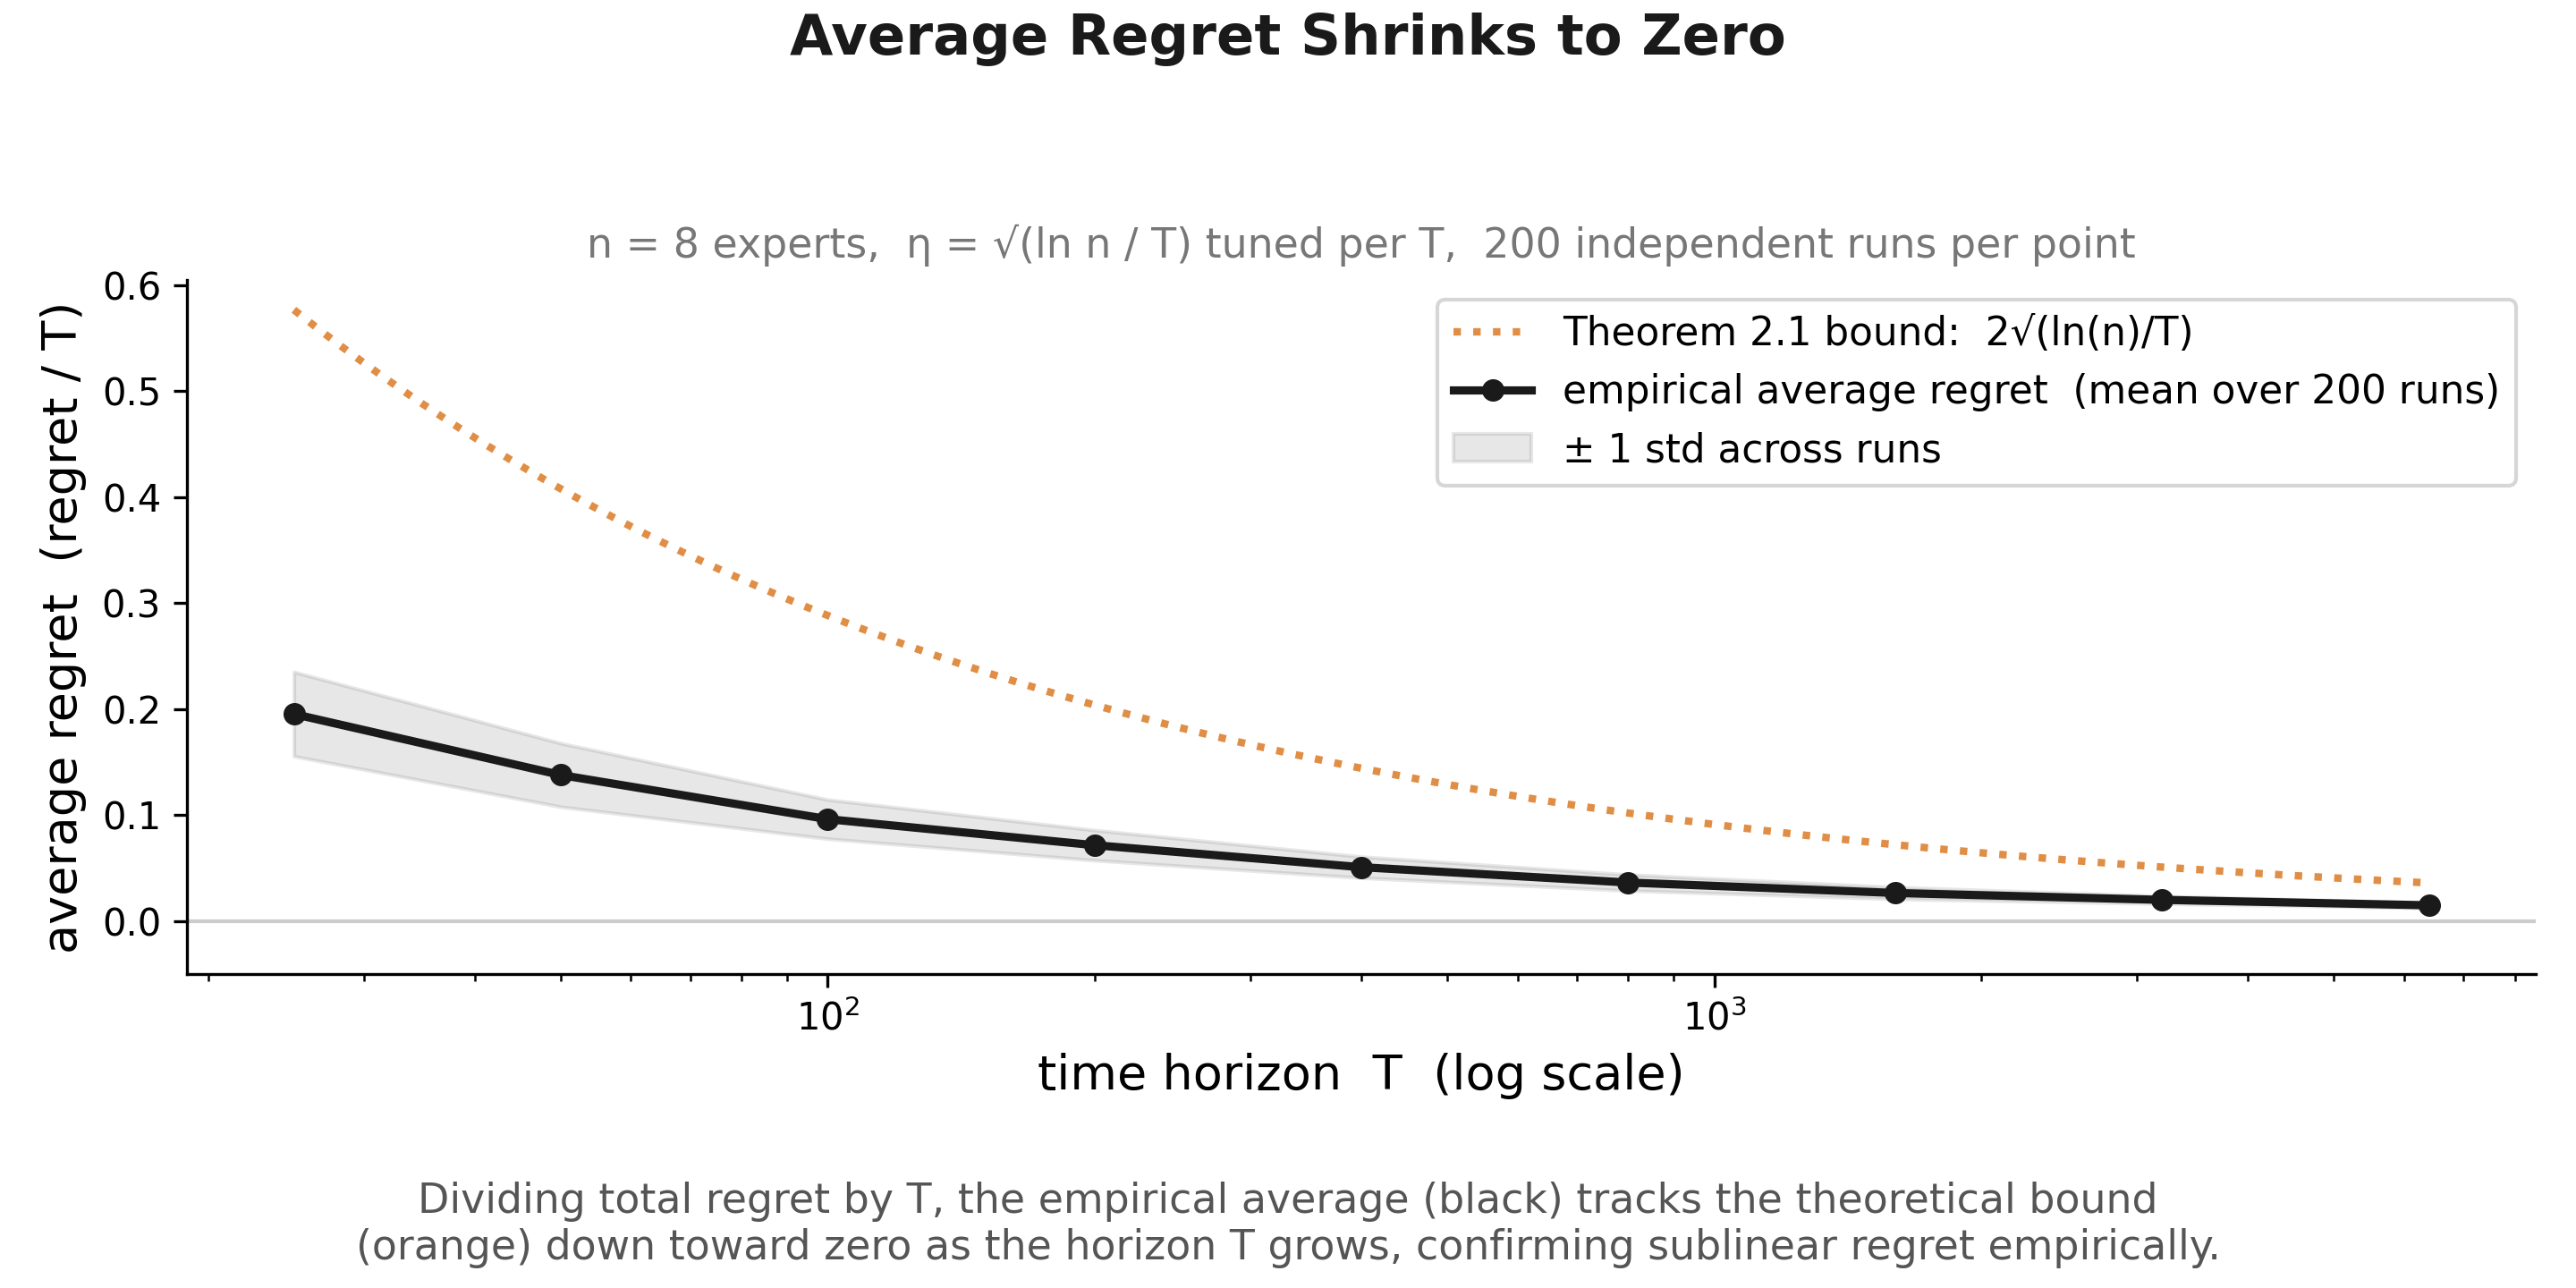
\includegraphics[width=\textwidth]{regret_convergence_plot.png}
\caption{Average regret $\regret_T/T$ of MW against the horizon $T$ ($n=8$, $\eta=\sq{\ln n/T}$ re-tuned per horizon, averaged over 200 random cost sequences), next to the bound $2\sq{\ln n/T}$.\\ \script{regret\_convergence\_plot.py}}
\label{fig:avg}
\end{minipage}
\end{figure}

\subsection{The average regret vanishes}

Dividing by $T$,
\[
\frac{\regret_T}{T} \;\le\; 2\sq{\frac{\ln n}{T}} \;\longrightarrow\; 0 \qquad (T\to\infty).
\]
This is the real content of the guarantee: not merely that the algorithm is close to the best decision, but that its per-round disadvantage vanishes as it gets more rounds to learn from, whatever $n$ is, because $n$ enters only through $\ln n$. Figure~\ref{fig:avg} measures it: the actual average regret of MW on random costs sits well below the bound and both go to zero.



% ================================================================== 6
\clearpage
\section{The lower bound: no algorithm beats the rate}
\label{sec:lower}

We have proved $\regret_T \le 2\sq{T\ln n}$ for MW. That is a fact about MW, not about the problem: perhaps a cleverer algorithm achieves $\sq{T}$ without the $\ln n$, or even $\ln T$, and our proof simply stopped short. The survey's Section~4 shows that this is not so.

\begin{theorem}[{adapted from \cite[Theorem~4.1 and its proof]{AHK12}}]
\label{thm:lower}
For every online algorithm (deterministic or randomised, adaptive or not) and every $n \ge 3$, $T \ge 4\ln(n-1)$, there is a sequence of costs $m^{(1)},\dots,m^{(T)} \in [-1,1]^n$ on which the algorithm's expected regret (over its own random choices) is at least
\[
\tfrac{1}{80}\sq{T \ln (n-1)} .
\]
\end{theorem}

The survey states the theorem asymptotically, as $\Omega(\sq{T\ln n})$; the explicit constant above is what its proof gives. Together with \eqref{eq:upper}, the optimal regret is $\Theta(\sq{T\ln n})$: MW has the right dependence on both $T$ and $n$, and only the constant in front could be improved.

\subsection{The method: let the adversary flip coins}

``Every algorithm'' is infinitely many algorithms, and we cannot design a bad input for each one by hand. The trick is to stop designing: let the costs be random, drawn from one fixed distribution that does not look at the algorithm at all, and compute the \emph{expected} regret of an arbitrary algorithm. If that expectation is at least $X$, then for that algorithm some particular outcome of the coins has regret at least $X$ --- an average cannot exceed its maximum. That outcome is a fixed cost sequence, which an adversary can simply play. This is the probabilistic method: a large average proves that a specific bad input exists, without finding it.

\subsection{The construction}

Decision $1$ costs exactly $\tfrac12$ in every round. Each of decisions $2,\dots,n$ costs $0$ or $1$ in every round, decided by an independent fair coin. So $t/2$ is the ``no-skill line'': decision $1$'s exact cost after $t$ rounds, and every coin's expected cost. Define the \emph{gap} of a decision after $t$ rounds as $t/2$ minus what it actually paid; decision $1$ has gap $0$ forever, a coin's gap wanders, and the largest gap among all decisions is exactly how much the best decision in hindsight beats the safe choice (Figure~\ref{fig:coins}).

\begin{figure}[htbp]
\centering
\includegraphics[width=\textwidth]{lucky_coin_plot.png}
\caption{The construction for $n=6$. Left: the cost matrix for 16 rounds (decision 1 pays $\frac12$; black $=1$, white $=0$ for the coins), the total each decision paid and its gap; the largest gap (decision 4, $+3$) is the best in hindsight. Right: the same gaps followed for 500 rounds; the luckiest coin's gap (orange) drifts away from decision 1's gap of zero (dashed).\\ \script{lucky\_coin\_plot.py}}
\label{fig:coins}
\end{figure}

\subsection{Every algorithm pays \texorpdfstring{$T/2$}{T/2}}

\begin{lemma}
\label{lem:half}
On the random costs above, every algorithm's expected total cost is exactly $T/2$.
\end{lemma}
\begin{proof}
Fix any algorithm. Its distribution $p^{(t)}$ is determined by rounds $1,\dots,t-1$ (and by the algorithm's own random bits). The costs $m^{(t)}$ of round $t$ are drawn independently of all of that, so conditioning on the past,
\[
\E\bigl[m^{(t)}\cdot p^{(t)} \,\big|\, \text{rounds } 1,\dots,t-1\bigr]
\;=\; \sum_i p^{(t)}_i\, \E\bigl[m^{(t)}_i\bigr]
\;=\; \sum_i p^{(t)}_i \cdot \tfrac12 \;=\; \tfrac12 .
\]
Decision $1$ costs $\frac12$ for sure and each coin costs $\frac12$ on average, so every mix costs $\frac12$ on average. Taking expectations and summing over $t$ gives $\E\bigl[\sum_t m^{(t)}\cdot p^{(t)}\bigr] = T/2$.
\end{proof}

Against fresh coins there is no skill: past information tells the algorithm nothing about the next flip, so no algorithm can beat the safe choice in expectation --- not because algorithms are bad, but because there is nothing to learn.

\subsection{Hindsight gets lucky}

The other side of the subtraction is what the best decision pays in hindsight. A coin decision's total cost over $T$ rounds is a sum of $T$ fair coins: a binomial with mean $T/2$ and standard deviation $\frac12\sq{T}$. Any one coin therefore lands about $\frac12\sq{T}$ away from $T/2$ by luck alone, up or down; and among $n-1$ independent coins, hindsight picks the luckiest. The maximum of many independent fluctuations grows like the square root of the logarithm of how many there are, which is where $\ln n$ enters.

\begin{lemma}[{\cite[Lemma~4.2]{AHK12}}]
\label{lem:lucky}
For $T \ge 4\ln(n-1)$, the expected cost of the best decision in hindsight satisfies
\[
\E\Bigl[\min_i \sum_{t=1}^{T} m^{(t)}_i\Bigr] \;\le\; \frac{T}{2} \;-\; \frac{1}{80}\sq{T\ln(n-1)} .
\]
\end{lemma}
\begin{proof}
Let $X_i = \sum_t m^{(t)}_i$; then $X_1 = T/2$ exactly and $X_i \sim \mathrm{Bin}(T,\frac12)$ for $i \ge 2$. Set $a = \frac14\sq{T\ln(n-1)}$; the assumption on $T$ gives $a \le T/8$. The survey uses the lower-tail estimate $\Pr[X_i \le T/2 - a] \ge \frac{1}{15}e^{-16a^2/T}$ for $0 \le a \le T/8$, which it takes from Matou\v{s}ek and Vondr\'ak\textquotesingle s lecture notes \cite{MV08}. This is an \emph{anti}-concentration bound for the binomial: the usual Chernoff bounds go the wrong way here, since we need the tail to be \emph{large}. With our $a$ this is $\Pr[X_i \le T/2 - a] \ge \frac{1}{15(n-1)}$. The $n-1$ coins are independent, so the probability that \emph{none} of them lands that low is at most
\[
\Bigl(1 - \tfrac{1}{15(n-1)}\Bigr)^{n-1} \;\le\; e^{-1/15} \;<\; 0.95 .
\]
Hence with probability at least $0.05$ the minimum is at most $T/2 - a$, and the minimum is never more than $T/2$ (decision 1 costs exactly $T/2$), so $\E[\min_i X_i] \le 0.05\,(T/2 - a) + 0.95\,(T/2) = T/2 - 0.05\,a = T/2 - \frac{1}{80}\sq{T\ln(n-1)}$.
\end{proof}

\begin{figure}[htbp]
\centering
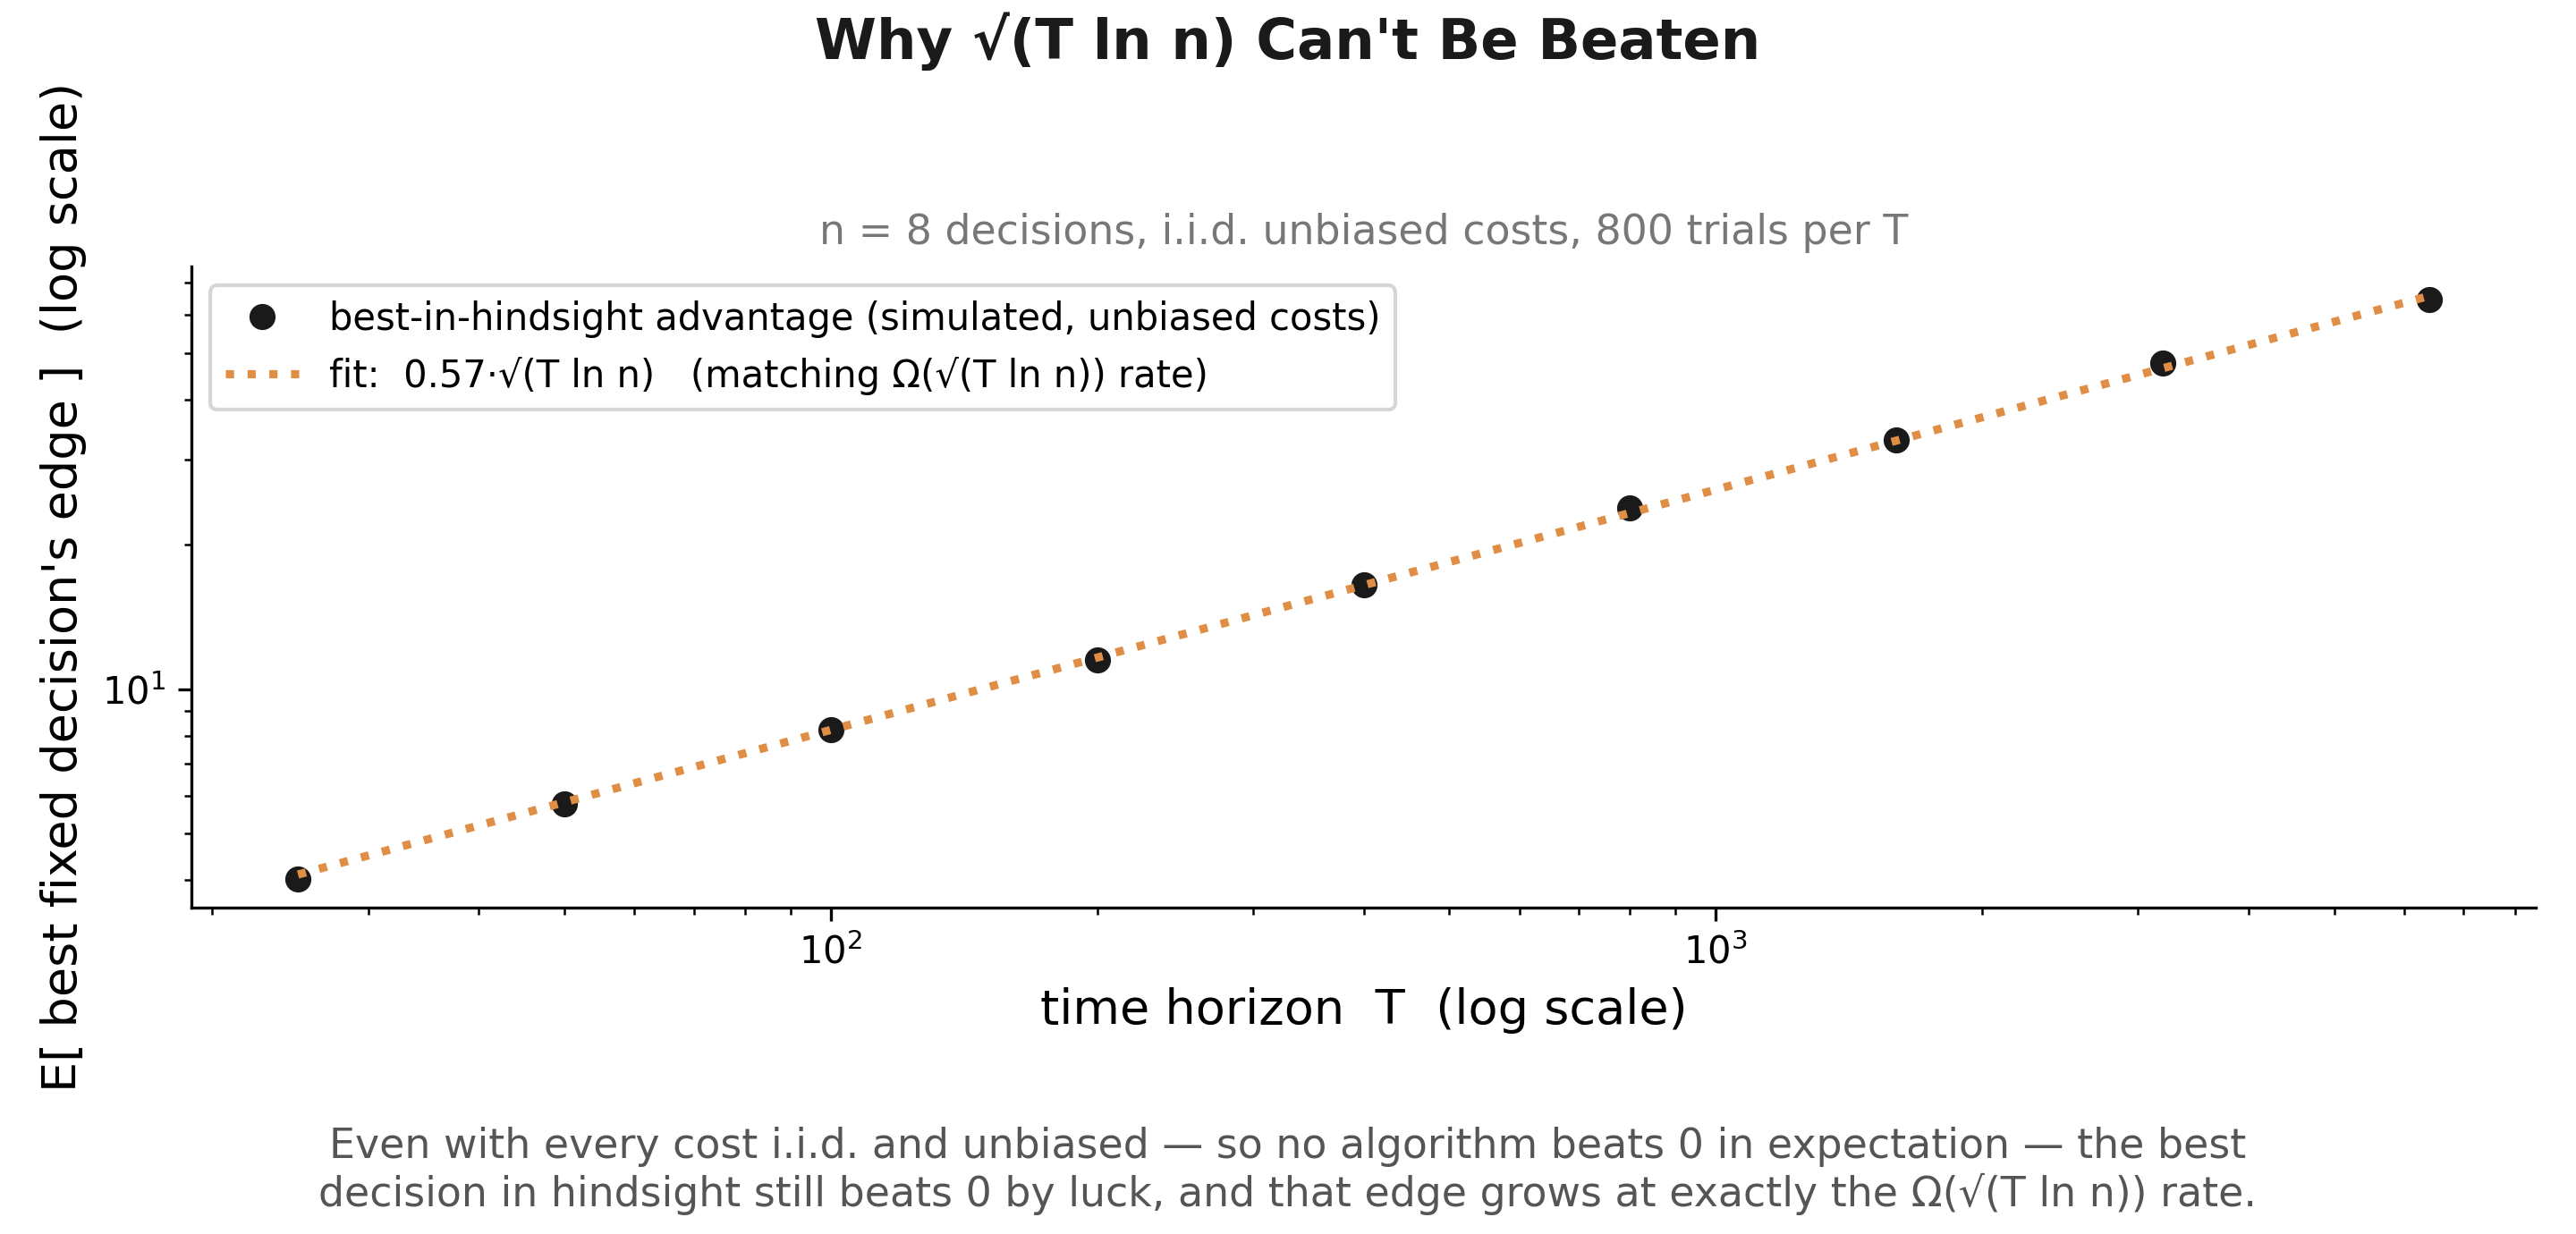
\includegraphics[width=0.7\textwidth]{lower_bound_plot.png}
\caption{Lemma~\ref{lem:lucky} measured: how far below $T/2$ the best of $n-1$ fair-coin decisions lands ($T = 500$, averaged over 3000 runs), against $n$ on a logarithmic axis, next to a scaled $\sq{\ln n}$. Hindsight's advantage grows with $n$, but only logarithmically.\\ \script{lower\_bound\_plot.py}}
\label{fig:lucky}
\end{figure}

\subsection{The rate is optimal}

\begin{proof}[Proof of Theorem~\ref{thm:lower}]
Subtract Lemma~\ref{lem:lucky} from Lemma~\ref{lem:half}:
\[
\E[\regret_T] \;=\; \E\Bigl[\sum_t m^{(t)}\cdot p^{(t)}\Bigr] - \E\Bigl[\min_i \sum_t m^{(t)}_i\Bigr]
\;\ge\; \frac{T}{2} - \Bigl(\frac{T}{2} - \frac{1}{80}\sq{T\ln(n-1)}\Bigr) \;=\; \frac{1}{80}\sq{T\ln(n-1)} .
\]
This is an expectation over the coins, so some fixed outcome of the coins --- a fixed cost sequence --- achieves at least this regret. (The costs used lie in $\{0,\frac12,1\} \subset [-1,1]$, so the sequence is admissible in Definition~\ref{def:problem}.)
\end{proof}

Put next to Section~\ref{sec:bound}: MW gets at most $2\sq{T\ln n}$, nobody gets less than $\frac{1}{80}\sq{T\ln(n-1)}$. Same $\sq{T}$, same $\sq{\ln n}$; on logarithmic axes the two bounds are parallel lines a constant factor apart (Figure~\ref{fig:tight}). The answer to the question that opened this section is: $2\sq{T\ln n}$ is the truth about the problem, not about our proof.

\begin{figure}[htbp]
\centering
\includegraphics[width=0.78\textwidth]{tight_bounds_plot.png}
\caption{The upper bound $2\sq{T\ln n}$ (Theorem~\ref{thm:mw}) and the lower bound $\frac{1}{80}\sq{T\ln(n-1)}$ (Theorem~\ref{thm:lower}) against $T$ on log--log axes, for $n=8$: the same slope $\frac12$, so the gap is only a constant factor.\\ \script{tight\_bounds\_plot.py}}
\label{fig:tight}
\end{figure}

% ================================================================== 7
\clearpage
\section{Two instantiations: AdaBoost and linear programs}
\label{sec:examples}

The meta-algorithm becomes a concrete algorithm once the four slots of Figure~\ref{fig:template} are filled. Table~\ref{tab:examples} fills them for two of the survey's applications; in both, the bottom row --- the update --- is character for character the one of Section~\ref{sec:algorithm}.

\begin{table}[htbp]
\centering
\small
\renewcommand{\arraystretch}{1.2}
\begin{tabular}{@{}>{\raggedright\arraybackslash}p{2.1cm}>{\raggedright\arraybackslash}p{5.7cm}>{\raggedright\arraybackslash}p{6.6cm}@{}}
\toprule
 & \textbf{AdaBoost} \cite{FS97}, \cite[Section~3.6]{AHK12} & \textbf{PST linear programs} \cite{PST95}, \cite[Section~3.3]{AHK12}\\
\midrule
a round     & run a weak learner on the current weighting & ask an oracle for a point $x$ satisfying the weighted constraint\\
a weight $w_i$ & how much training example $i$ still matters & how much constraint $i$ still matters\\
a cost $m_i$ & $1$ if the hypothesis got example $i$ right, $0$ if wrong & $(A_i x - b_i)/\rho$: the slack of constraint $i$, scaled by its width $\rho$\\
the goal    & focus the next learner on the hard examples & reach approximate feasibility\\
the rate $\eta$ & $\gamma$, the weak learner's edge over guessing & $\varepsilon/4\ell$, set by the accuracy wanted\\
the update  & $w_i \leftarrow w_i(1-\eta m_i)$ & $w_i \leftarrow w_i(1-\eta m_i)$\\
\bottomrule
\end{tabular}
\caption{Two instantiations of the same update rule.}
\label{tab:examples}
\end{table}

\paragraph{AdaBoost.}
Swap ``decision'' for ``training example''. An example the current hypothesis classifies correctly has cost $1$, so its weight shrinks; an example that is misclassified keeps its full weight and becomes relatively louder next round, forcing the next weak learner to concentrate on exactly the examples it keeps getting wrong. The weak learner is promised an edge $\gamma$ over random guessing every round, and that promise plays the role of the learning rate. The sandwich argument of Section~\ref{sec:proof} then bounds the number of examples the final combined classifier gets wrong, which is Freund and Schapire's boosting theorem \cite{FS97}.

\paragraph{Plotkin--Shmoys--Tardos.}
Swap ``decision'' for ``constraint'' of a linear program $Ax \ge b$, $x \in P$. Each round an oracle is asked for a point $x \in P$ satisfying only the single \emph{weighted} constraint $p^{(t)\top}Ax \ge p^{(t)\top}b$, which is easy; the cost of constraint $i$ is its slack $(A_ix - b_i)/\rho$, normalised by the width $\rho$ so that costs lie in $[-1,1]$ (the parameter $\ell$ bounds how negative the slack can be). A satisfied constraint has positive cost and its weight shrinks --- we stop worrying about it --- while a violated constraint gains weight and pulls the next candidate back. Theorem~\ref{thm:mw} then says that the average of the points returned satisfies every constraint up to $\varepsilon$ after $O(\ell\rho\ln n/\varepsilon^2)$ rounds \cite[Section~3.3]{AHK12}.

% ================================================================== 8
\clearpage
\section{Nature got there first: evolution runs the same update}
\label{sec:nature}

The last instantiation is not from computer science. Chastain, Livnat, Papadimitriou and Vazirani \cite{CLPV14}, citing the survey, showed that the dynamics of natural selection under sexual reproduction are, in the regime of weak selection, exactly the Multiplicative Weights update: each gene plays the role of a decision maker, its alleles are the decisions, the fraction of the population carrying an allele is its weight, and the allele's fitness is minus its cost.

\paragraph{The setting.}
A population of organisms; one gene, which comes in variants --- \emph{alleles} --- $A,B,C,D$; every organism carries one of them. Fitness is reproductive success: a carrier of allele $i$ leaves, on average, $1 + s\,f_i$ offspring, where $f_i$ is the allele's relative fitness and $s$ is the strength of selection. After one generation the share of allele $i$ in the population is therefore
\begin{equation}
\label{eq:selection}
x_i \;\longleftarrow\; \frac{x_i\,(1 + s f_i)}{\sum_j x_j\,(1 + s f_j)} ,
\end{equation}
the shares having been renormalised to sum to one (Figure~\ref{fig:population}).

\begin{figure}[htbp]
\centering
\includegraphics[width=\textwidth]{population_plot.png}
\caption{One generation of selection: 100 organisms (one dot each, coloured by allele) before and after, with the fitness of each allele. Allele $C$, the fittest, grows from 25\% to 29\%. (Selection strength exaggerated to $s=5$ so that one generation is visible; the text and Figure~\ref{fig:evolution} use weak selection.)\\ \script{population\_plot.py}}
\label{fig:population}
\end{figure}

\paragraph{The correspondence.}
Compare \eqref{eq:selection} with the MW algorithm: $x_i(1+sf_i)$ is $w_i(1-\eta m_i)$ with cost $m_i = -f_i$ and learning rate $\eta = s$, and the renormalisation is exactly the play line $p_i = w_i/\Phi$. Table~\ref{tab:evolution} lines the two up. The claim of \cite{CLPV14} is stronger than this single-locus identity: with many genes and recombination, under weak selection (small $s$), the joint dynamics are equivalent to every gene running MW in a coordination game whose payoffs are the fitness contributions --- and Theorem~\ref{thm:mw} applies verbatim with $\eta = s$: over $T$ generations each gene's cumulative fitness is within $sT + (\ln n)/s$ of what the best fixed allele would have achieved. Sexual reproduction has been running this update for over a billion years. (The interpretation of what the population is ``optimising'' was debated afterwards \cite{MP15}; the correspondence between the update rules is exact.)

\begin{table}[htbp]
\centering
\small
\renewcommand{\arraystretch}{1.15}
\begin{tabular}{@{}lll@{}}
\toprule
 & \textbf{Multiplicative Weights} & \textbf{Evolution} \cite{CLPV14}\\
\midrule
a round & one update & one generation\\
a weight & how much we trust decision $i$ & how common allele $i$ is\\
a cost & what decision $i$ cost us & minus its fitness\\
the goal & track the best decision & the population adapts\\
the rate $\eta$ & chosen by us & $s$, the strength of selection\\
the update & $w_i \leftarrow w_i(1-\eta m_i)$ & $x_i \leftarrow x_i(1 + s f_i)$\\
\bottomrule
\end{tabular}
\caption{The same table, one more time.}
\label{tab:evolution}
\end{table}

\begin{figure}[htbp]
\centering
\includegraphics[width=0.9\textwidth]{evolution_plot.png}
\caption{Allele shares over 260 generations under \eqref{eq:selection} with fitnesses $(0, 0.03, 0.06, 0.02)$ and $s = 0.5$: the fittest variant takes over, the others fade --- the same shape as the stock run of Figure~\ref{fig:stocks}, because it is the same update.\\ \script{evolution\_plot.py}}
\label{fig:evolution}
\end{figure}

% ================================================================== 9
\clearpage
\section{Influence: what has been built on the survey}
\label{sec:influence}

The survey's own claim is that the reweighting scheme deserves to be a basic algorithmic tool on the footing of divide-and-conquer or dynamic programming. The record since 2012 supports it: the paper is cited across computer science and beyond. Figure~\ref{fig:bowtie} shows a few of the citing works, chosen to span fields.

\begin{figure}[htbp]
\centering
\includegraphics[width=\textwidth]{bowtie_plot.png}
\caption{Found three times, unified once, cited everywhere: the three predecessors feeding into the 2012 survey, and six of the papers that cite it, across biology, privacy, quantum computing, machine learning and algorithms.\\ \script{bowtie\_plot.py}}
\label{fig:bowtie}
\end{figure}

\begin{itemize}[itemsep=3pt]
  \item \emph{Differential privacy.} Hardt and Rothblum's Private Multiplicative Weights mechanism \cite{HR10} answers a long sequence of statistical queries on a database while preserving differential privacy: it maintains a synthetic database as a weight vector over the data universe and applies the MW update only on queries the current synthetic answer gets badly wrong; the regret bound turns into a bound on the number of such updates, and hence on the privacy cost.
  \item \emph{Quantum algorithms.} Van Apeldoorn, Gily\'en, Gribling and de Wolf \cite{vAGGdW17} obtain quantum speed-ups for solving semidefinite programs by implementing the survey's Matrix Multiplicative Weights framework \cite[Section~5]{AHK12} with quantum Gibbs sampling.
  \item \emph{Language-model training.} Aioli \cite{Aioli25} studies how to mix data sources when training a language model and proves that three published, seemingly different data-mixing methods are each a single exponentiated-gradient (multiplicative-weights) update on the mixture proportions, differing only in how the loss signal is estimated.
  \item \emph{Graph algorithms.} Nguyen and Ene \cite{NE24} use MW as the outer loop of fast algorithms for densest-subgraph problems; Cao et al.\ \cite{Cao25} solve the cluster LP for correlation clustering in sublinear time, again with a multiplicative-weights core.
  \item \emph{Biology.} The evolution paper of Section~\ref{sec:nature} \cite{CLPV14}.
\end{itemize}

Within learning theory the idea also kept evolving along the lines the survey pointed to. Online convex optimisation \cite{Zinkevich03} replaces the $n$ discrete decisions by a point in a convex set; the discrete problem of Definition~\ref{def:problem} is the special case where the set is the probability simplex, and the $\ln n$ in the bound becomes a measure of the set's size. AdaHedge \cite{AdaHedge14} removes the one practical blemish of Section~\ref{sec:bound}, the need to know $T$ in advance to set $\eta = \sq{\ln n/T}$, by tuning $\eta$ on the fly while keeping the same $O(\sq{T\ln n})$ guarantee. Hazan's monograph \cite{Hazan16}, by one of the survey's authors, treats the material of Sections~\ref{sec:algorithm}--\ref{sec:bound} as a single early chapter of a much larger theory.

% ================================================================== 10
\clearpage
\section{Summary}

The journey of this seminar, in six lines.
\emph{History}: the same four-line update was found in learning theory, optimisation and boosting before anyone noticed it was one algorithm.
\emph{The problem}: $n$ decisions, adversarial costs, and regret --- the distance from the best single decision in hindsight --- as the yardstick (Definition~\ref{def:problem}).
\emph{The algorithm}: $w_i \leftarrow w_i(1-\eta m_i)$, renormalise, repeat.
\emph{The proof}: one potential $\Phi = \sum_i w_i$, squeezed from below by one decision's costs and from above by the algorithm's, then logarithms (Theorem~\ref{thm:mw}).
\emph{The limits}: $\regret_T \le 2\sq{T\ln n}$, and no algorithm at all beats $\Omega(\sq{T\ln n})$ (Theorem~\ref{thm:lower}).
\emph{Nature}: selection on alleles is the same update, with fitness for minus cost and selection strength for $\eta$.

The real contribution of the survey is not the algorithm --- most of its applications existed already --- but the observation that one potential function and one proof built around it are enough to derive all of them at once, and the lower bound showing that this proof is not merely convenient but tight. One rule, one proof, and a field that stopped reinventing it.

% ================================================================== references
\clearpage
\begin{thebibliography}{99}
\small\raggedright\setlength{\itemsep}{2pt}

\bibitem{AHK12} S.~Arora, E.~Hazan and S.~Kale. The Multiplicative Weights Update Method: a Meta-Algorithm and Applications. \emph{Theory of Computing} 8(6):121--164, 2012. \url{https://theoryofcomputing.org/articles/v008a006/v008a006.pdf}

\bibitem{Littlestone88} N.~Littlestone. Learning quickly when irrelevant attributes abound: a new linear-threshold algorithm. \emph{Machine Learning} 2(4):285--318, 1988. \url{https://doi.org/10.1007/BF00116827}

\bibitem{PST95} S.~A.~Plotkin, D.~B.~Shmoys and \'E.~Tardos. Fast approximation algorithms for fractional packing and covering problems. \emph{Mathematics of Operations Research} 20(2):257--301, 1995 (preliminary version in FOCS 1991). \url{https://doi.org/10.1287/moor.20.2.257}

\bibitem{FS97} Y.~Freund and R.~E.~Schapire. A decision-theoretic generalization of on-line learning and an application to boosting. \emph{Journal of Computer and System Sciences} 55(1):119--139, 1997. \url{https://doi.org/10.1006/jcss.1997.1504}

\bibitem{CLPV14} E.~Chastain, A.~Livnat, C.~Papadimitriou and U.~Vazirani. Algorithms, games, and evolution. \emph{Proceedings of the National Academy of Sciences} 111(29):10620--10623, 2014. \url{https://doi.org/10.1073/pnas.1406556111}

\bibitem{MP15} R.~Meir and D.~Parkes. On sex, evolution, and the multiplicative weights update algorithm. \emph{Proceedings of AAMAS 2015}, 929--937. \url{https://arxiv.org/abs/1502.05056}

\bibitem{MV08} J.~Matou\v{s}ek and J.~Vondr\'ak. The probabilistic method. Lecture notes, Charles University, 2008. \url{https://kam.mff.cuni.cz/~matousek/prob-ln.pdf.gz}

\bibitem{HR10} M.~Hardt and G.~N.~Rothblum. A multiplicative weights mechanism for privacy-preserving data analysis. \emph{Proceedings of FOCS 2010}, 61--70. \url{https://doi.org/10.1109/FOCS.2010.85}

\bibitem{vAGGdW17} J.~van Apeldoorn, A.~Gily\'en, S.~Gribling and R.~de Wolf. Quantum SDP-solvers: better upper and lower bounds. \emph{Proceedings of FOCS 2017}, 403--414. \url{https://doi.org/10.1109/FOCS.2017.44}

\bibitem{Aioli25} M.~F.~Chen, M.~Y.~Hu, N.~Lourie, K.~Cho and C.~R\'e. Aioli: a unified optimization framework for language model data mixing. \emph{Proceedings of ICLR 2025}. \url{https://arxiv.org/abs/2411.05735}

\bibitem{NE24} T.~D.~Nguyen and A.~Ene. Multiplicative weights update, area convexity and random coordinate descent for densest subgraph problems. \emph{Proceedings of ICML 2024}. \url{https://proceedings.mlr.press/v235/nguyen24e.html}

\bibitem{Cao25} N.~Cao, V.~Cohen-Addad, E.~Lee, S.~Li, D.~Rasmussen~Lolck, A.~Newman, M.~Thorup, L.~Vogl, S.~Yan and H.~Zhang. Solving the correlation cluster LP in sublinear time. \emph{Proceedings of STOC 2025}, 1154--1165. \url{https://doi.org/10.1145/3717823.3718181}

\bibitem{Zinkevich03} M.~Zinkevich. Online convex programming and generalized infinitesimal gradient ascent. \emph{Proceedings of ICML 2003}, 928--936. \url{https://www.aaai.org/Papers/ICML/2003/ICML03-120.pdf}

\bibitem{AdaHedge14} S.~de~Rooij, T.~van~Erven, P.~D.~Gr\"unwald and W.~M.~Koolen. Follow the leader if you can, hedge if you must. \emph{Journal of Machine Learning Research} 15(37):1281--1316, 2014. \url{https://jmlr.org/papers/volume15/rooij14a/rooij14a.pdf}

\bibitem{Hazan16} E.~Hazan. Introduction to online convex optimization. \emph{Foundations and Trends in Optimization} 2(3--4):157--325, 2016. \url{https://doi.org/10.1561/2400000013}

\bibitem{Repo} T.~Idelson. MW-Seminar: code and figure scripts for this seminar. GitHub repository, 2026. \url{https://github.com/bental1/MW-Seminar}

\end{thebibliography}

\end{document}
